\documentclass{../template/texnote}

\title{\textbf{\capitalisewords{The Little Green Men in Space}}}

\begin{document}
    \maketitle \currentdoc{note}
    %<*note>
Radios, apart from being a fun and useful piece of technology, are critical to almost all communication in our daily lives. Did you know that cellphones use radio waves for communicating with each other? Or that radio waves are used in WiFi or Bluetooth communications?
If you have ever used a traditional radio receiver for tuning into radio stations you have seen that between the designated stations which broadcast programs all you get is noise. If so 
 why do we use radio waves in astronomy? Do we expect radio stations to be run by the denizens of galaxies near or far? Turns out that we did find such a broadcast when we listened very carefully into the depths of space using powerful radio receivers. Lets find out what that was all about and more interesting things about radio astronomy in this article.
\section{What are radio waves?}
Radios were all the rage in the not so distant past. Radio waves revolutionized communication and entertainment in the early 20th century. During world war II radios played a critical role in military communication.  In the 1960s and 1970s, FM radio gained popularity for its superior sound quality. Although today radio has mostly fallen out of fashion in the entertainment industry they are critical to most of our modern communication. Television broadcasting, satellite communications and even the GPS system used for navigation all make use of radio waves. Modern methods of wireless communication such as cellphone communication, WiFi and Bluetooth would be unthinkable without radio waves. Radars that make use of radio waves are used for various applications. Medical imaging is another area which makes use of radio waves. Radio Frequency Identification (RFID) tags are used in  a variety of places and are fast becoming common place.
\section{Why did radio waves have to be discovered?}
Life that evolved on earth developed mechanisms to detect visible light, the things that we call eyes, probably because of the interplay of various factors. The visible spectrum corresponds to wavelengths that are easily absorbed and reflected by the materials found in nature, such as water, plants, and animals. This allows organisms to perceive and distinguish objects in their environment, such as food, predators, and potential mates. Furthermore, the Sun emits a large amount of radiation in the visible portion of the spectrum, which provides the energy for photosynthesis and drives the Earth's climate and weather patterns. The other parts of the electromagnetic spectrum remained largely hidden from us. After Maxwell predicted the existence of electromagnetic waves in 1864, Heinrich Hertz produced radio waves in the late 1880s to experimentally demonstrate their existence. The discovery of other kinds of EM waves such as X-rays soon followed. The discovery of radio waves sparked a revolution in science and technology. The telegraph which was the primary means of long distance communication now had a wireless alternative. Other uses of these newly discovered waves soon followed. Before we learn more about radio waves it is essential to have a good understanding of what electromagnetic radiation is and how it is produced both naturally and by artificial means.
\section{What is electromagnetic radiation?}
Stationary electric charges produce electric fields, whereas moving electric charges produce both electric and magnetic fields. When a charge accelerates or undergoes a change in its magnitude (charge or discharge) a disturbance in the electromagnetic field is produced. This is often a pulse of electromagnetic radiation that can self propagate outwards at the speed of light. This is very much like how you create a ripple on the surface of a still pond by throwing a stone into it. In order to create a steady wave as opposed to just a pulse you need to have a source that oscillates regularly. The frequency of such a wave is decided by the frequency of the source of the disturbance and it is this frequency that decides the properties of the radiation. The frequency also decides the energy of the radiation and often our ability to detect the radiation. Thus electromagnetic radiation falls on a broad spectrum depending on the frequency from low frequency radio waves to the highest frequency gamma rays.
\section{What are the mechanisms that create EM waves?}
The different possible ways in which you can accelerate charges leads to the different source of electromagnetic radiation. In general you have thermal and non-thermal sources of electromagnetic waves. Examples of thermal radiation include Continuous spectrum emissions related to the temperature of the object or material and Specific frequency emissions from neutral hydrogen and other atoms and molecules. Examples of non-thermal mechanisms include emissions due to synchrotron radiation and Amplified emissions due to astrophysical masers. In a hot object be it solid, liquid or gas the constituent particles are always in accelerated motion either due to vibration or collisions. As a result electromagnetic radiation is emitted at all possible frequencies in the spectrum but the amount of energy in each frequency depends on the temperature of the object.
\section{A radio universe}
We already saw several man-made source of radio waves. What are some of the natural sources of radio waves? On Earth, the discharge of electricity in lightnings is a source of radio waves. The bigger source of radio waves is the Sun. Solar flares and coronal mass ejections can produce intense bursts of radio waves that can be a threat to our communication and navigational systems. These radio waves are produced through a process called plasma emission. Plasma, which is a highly ionized gas, can produce radio waves when it is disturbed by energetic charged particles. In the case of solar flares and CMEs, the charged particles accelerated by the events can create disturbances in the plasma that lead to the emission of radio waves.


In 1932, Karl Jansky a radio engineer at the Bell Telephone Laboratories was assigned to study radio interference from thunderstorms. During his investigations he found static that he concluded to be of extraterrestrial origin and not related to the static from thunderstorms. Upon further investigations he discovered the source of the static to be the Milky way galaxy and opened up radio astronomy as a field of study. The typical astrophysical sources of radio waves are dark dust clouds (refer Fig \ref{fig:radio_table}). Visible stars radiate a lot of electromagnetic energy by definition in the visible region of the spectrum. Part of the energy has to be in the microwave (short wave radio) part of the spectrum, and that is the part astronomers study using radio telescopes. Despite their temperatures however all visible stars do not make for good radio frequency sources. We can detect stars at radio frequencies only if they emit by non-thermal mechanisms, or if they are in our solar system (that is, our sun), or if there is gas beyond the star which is emitting (for example, a stellar wind).

\begin{figure}
    \centering
    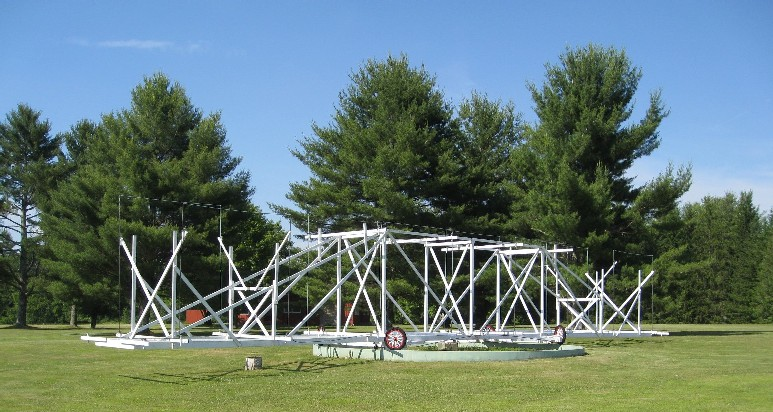
\includegraphics[scale=1.4]{Linn/Janksy_Karl_radio_telescope.jpg}
    \caption{Full-size replica of the first radio telescope, Jansky's dipole array of 1932, preserved at the US Green Bank Observatory in Green Bank, West Virginia. Image Credit: Wikipedia}
    \label{fig:jansky}
\end{figure}

\begin{figure}
    \centering
    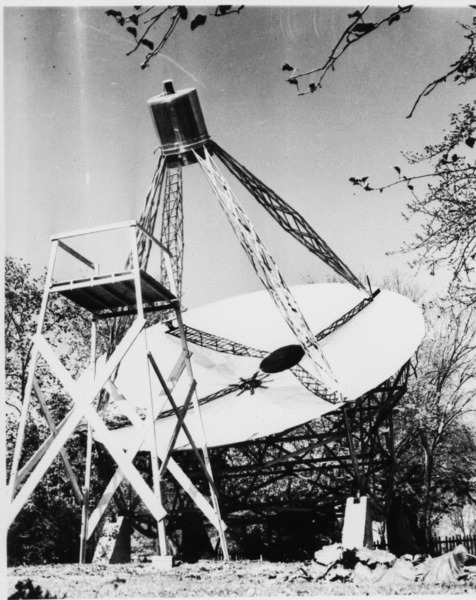
\includegraphics[scale=0.56]{Linn/476px-Grote_Antenna_Wheaton.jpg}
    \caption{The first parabolic "dish" radio telescope by Grote Reber, Wheaton, Illinois, 1937. Image Credit: Wikipedia}
    \label{fig:reber}
\end{figure}

\begin{figure}
    \centering
    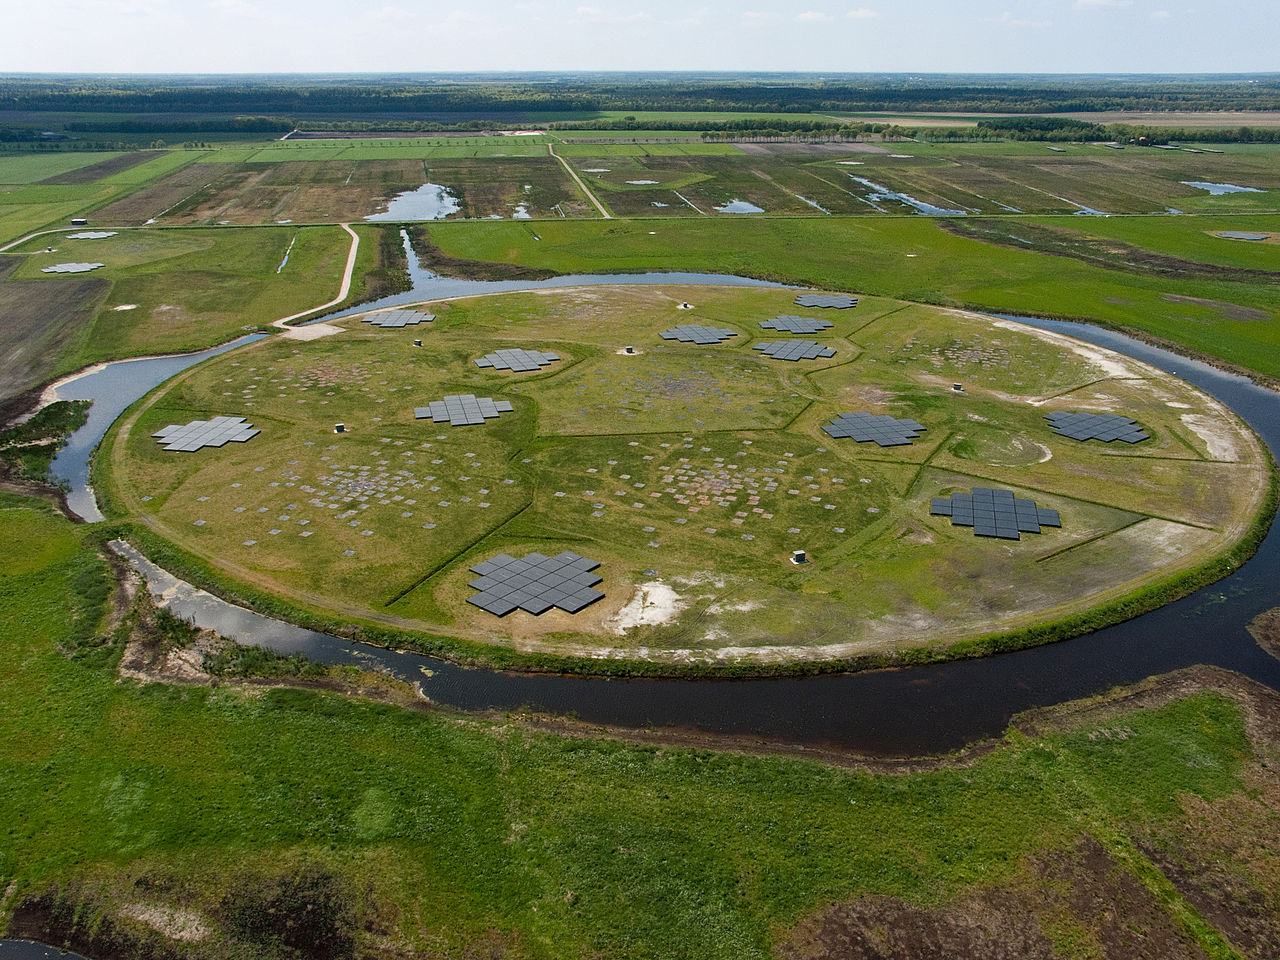
\includegraphics[scale=0.9]{Linn/1280px-LOFAR_Superterp.jpg}
    \caption{The LOFAR core ("superterp") near Exloo, Netherlands. The bridges give an idea of the scale. Image Credit: Wikipedia}
    \label{fig:radio_lofar}
\end{figure}

\begin{figure}
    \centering
    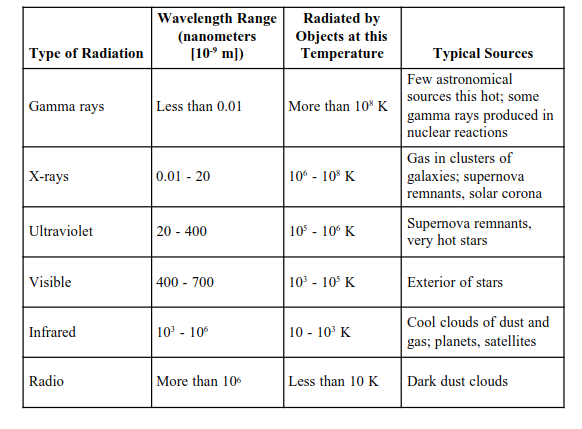
\includegraphics[scale=0.6]{Linn/26_641fd632-e947-4bd1-aa1b-8b3de855731c_1679808050374.png}
    \caption{Table showing different astrophysical sources of radio waves}
    \label{fig:radio_table}
\end{figure}

\section{The story of the Little Green Men}
In 1967, Jocelyn Bell, a postgraduate student at Cambridge University, was working with her supervisor, Antony Hewish, on a radio telescope designed to study quasars. While analyzing the data from the telescope, she noticed a strange signal that was pulsing regularly. The signal differed from the generally chaotic nature of most cosmic phenomenon. Additionally the signal was of a very specific radio frequency, whereas most natural sources typically radiate across a wider range. These things led the research team to contemplate the possibility of having found an artificially created signal from an extraterrestrial intelligent species. They even dubbed the source as LGM 1 or Little Green Men 1. However their discovery later turned out to be the first detection of a pulsar. Pulsars spin rapidly, while simultaneously radiating opposing beams of radio waves out into space. The setup is similar to a lighthouse that spins around one up-and-down axis and radiates two beams of light from a second axis. Antony Hewish and Martin Ryle received the Nobel Prize in physics in 1974 for their work in radio astronomy and pulsars.
\begin{figure}
    \centering
    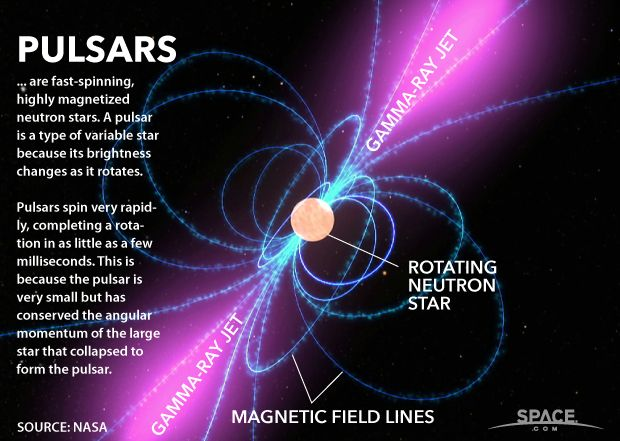
\includegraphics[scale=0.6]{Linn/B6ZF4muxXJv9AUJ8xcRfbf-1024-80.jpg}
    \caption{Graphical depiction of Pulsars. Image Credit: Space.com}
    \label{fig:pulsars}
\end{figure}

\section{Why do we need radio astronomy?}
 Radio astronomy allows us to detect and study phenomena that emit little or no visible light, such as pulsars and black holes. And in this way they act as complimentary source of information. Radio waves can pass through clouds of dust and gas, allowing astronomers to observe objects that are obscured from view in optical telescopes. They can travel vast distances without being absorbed, making it possible to study objects at the farthest reaches of the universe. Finally radio telescopes can collect data continuously, day and night, providing astronomers with a wealth of information about the universe around the clock
Apart from the discovery of pulsar radio astronomy has resulted in several remarkable astronomical discoveries. The discovery of the cosmic microwave background radiation was made using the radio telescope in New Jersey. It provided irrefutable evidence for the Big Bang model of the origin of the universe. More recently in 2019, the Event Horizon Telescope project produced the first-ever image of a black hole. The image was created using data from a network of radio telescopes around the world.


\section{The challenges in radio astronomy}
Radio astronomy is also a very technically demanding field. The building of large radio telescope involves complex engineering and construction challenges, and maintaining and operating these instruments requires highly trained professionals. Radio waves are relatively weak and can be easily overwhelmed by noise from various sources, including terrestrial sources such as cell phone towers and other electronic devices. Thus radio telescopes must be carefully designed and located in remote areas to minimize interference. Scattering and distortion of radio signal by the atmosphere is another area of concern. Radio astronomers must carefully calibrate their instruments and develop sophisticated data analysis techniques to separate the desired signal from the background noise. These and other efforts in radio astronomy often involves analyzing vast amounts of data, which requires sophisticated computer algorithms and data processing techniques.

\begin{figure}
    \centering
    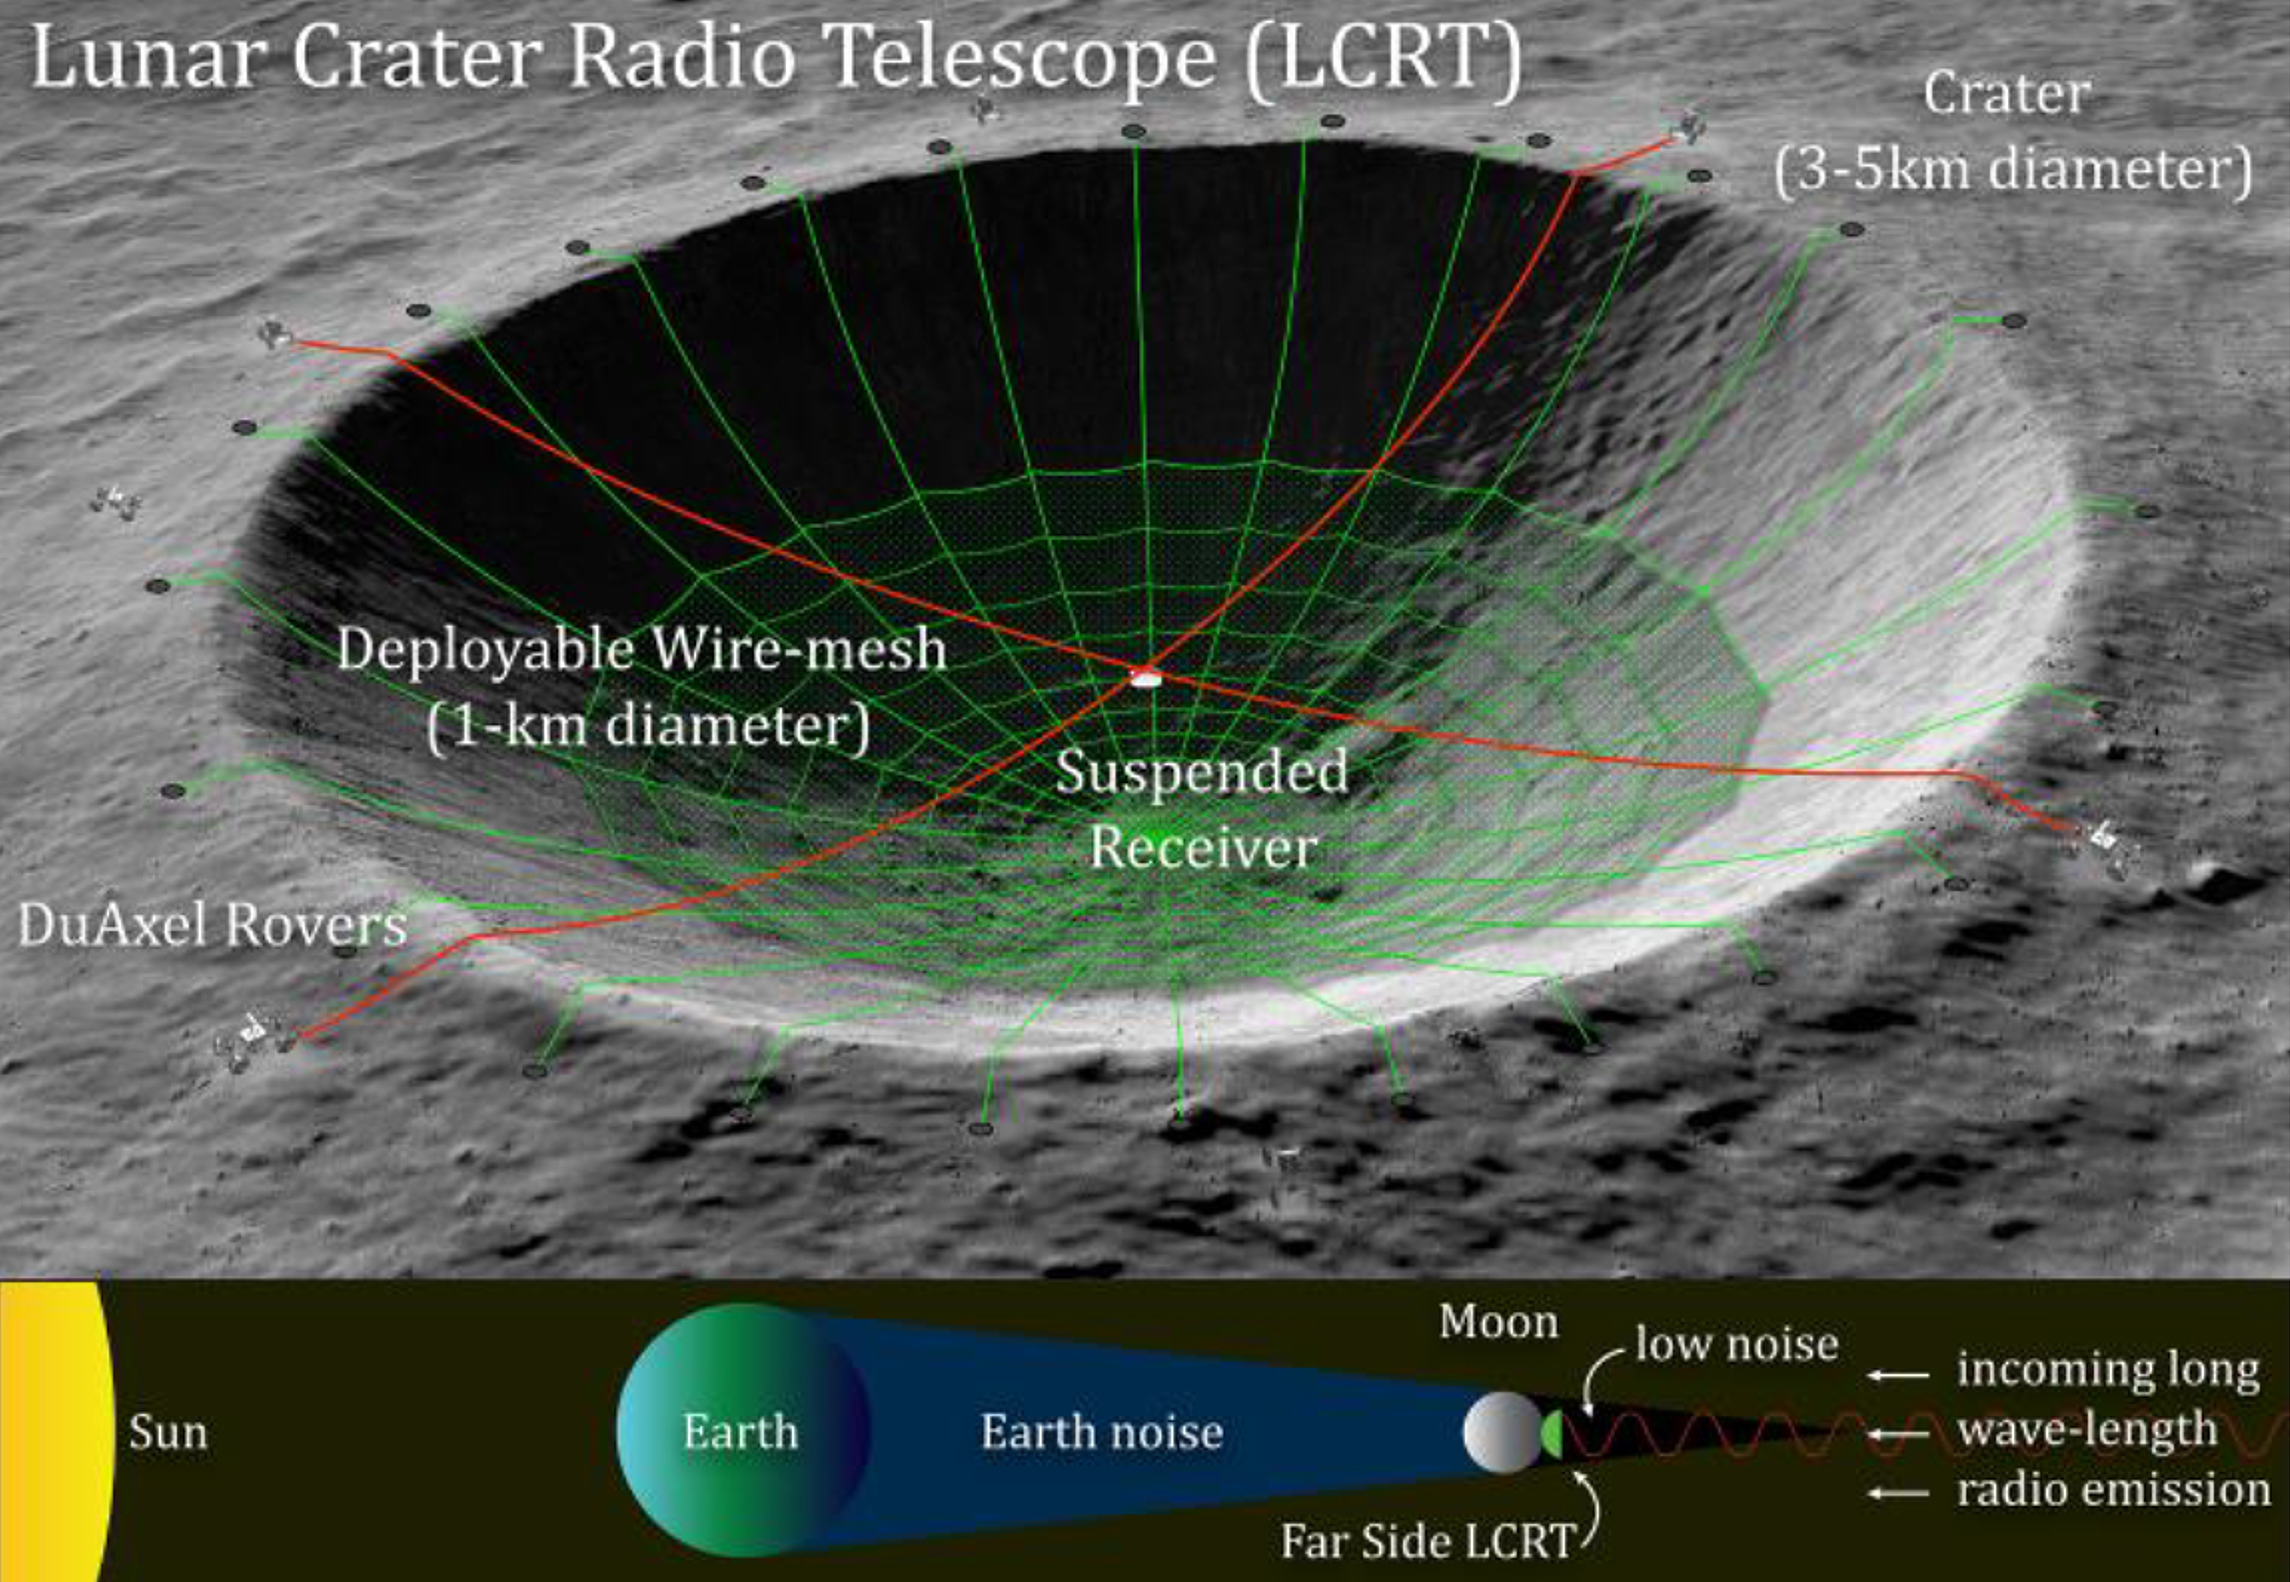
\includegraphics[scale=0.19]{Linn/niac2020_bandyopadhyay.jpg}
    \caption{The proposed Lunar Crater Radio Telescope (LCRT) on the Far-Side of the Moon. Image Credit:NASA}
    \label{fig:radio_moon}
\end{figure}

\section{References}
\begin{enumerate}
    \item \href{https://www.space.com/38916-pulsar-discovery-little-green-men.html}{Little Green Men? Pulsars Presented a Mystery 50 Years Ago}
    \item \href{https://en.wikipedia.org/wiki/Cosmic_microwave_background}{Cosmic microwave background}
    \item \href{https://en.wikipedia.org/wiki/PSR_B1919%2B21}{PSR B1919+21}
	\item \href{https://www2.jpl.nasa.gov/radioastronomy/radioastronomy_all.pdf}{Basics of Radio Astronomy by Diane Fisher Miller}
\end{enumerate}
    %</note>
    \printbibliography
\end{document}
